\section{Breadth-first Search}
\index{breadth-first search}
\index{search!breadth-first}
\index{BFS}

Breadth-first search is a method of searching an unweighted graph of nodes.
Ultimately, the search is implemented using a queue to visit nodes in the immediate neighborhood of the current node (nodes that are separated by only one edge) before branching out to explore nodes further away.
As each node is seen, it is marked as visited.
Only nodes that have not been marked as visited are added to the queue.
Using this technique, one can find the shortest path from a given node to another node.
The running time of the algorithm can be described as $O(m + n)$ for a given graph containing $m$ nodes and $n$ edges.

\begin{figure}[h]
	\centering
	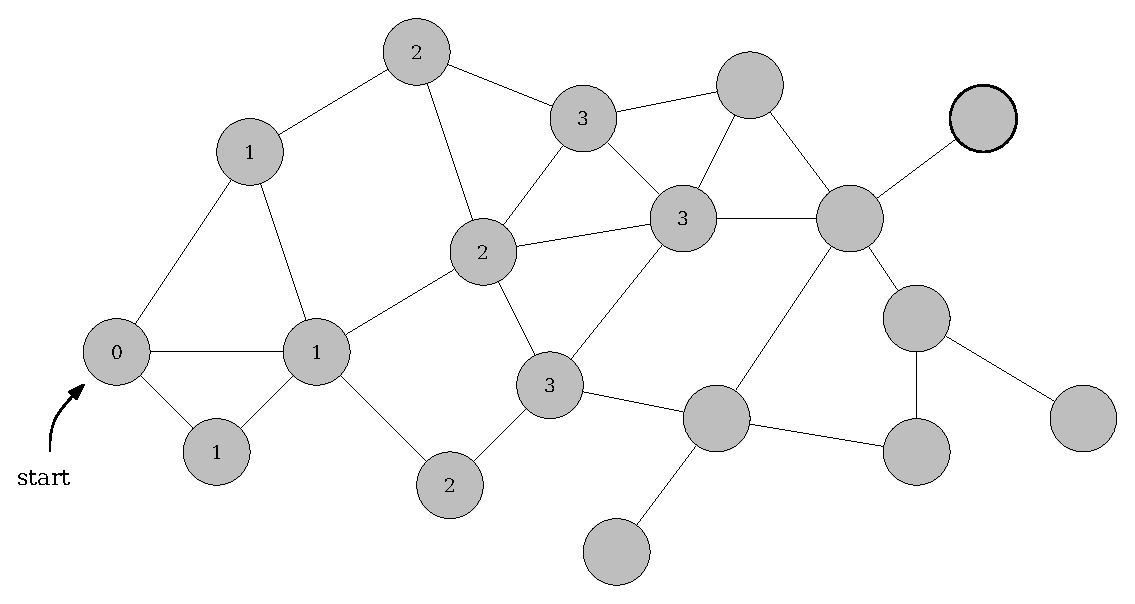
\includegraphics[width=0.6\textwidth]{./algorithms/breadth-first-search/partial-bfs}
	\caption{\small A partially completed breadth-first search on a graph with no particular target node.}
\end{figure}

\subsection{Applications}

\begin{itemize}
	\item Searching graphs with unit edges.
		Graphs with weighted edges should use the Dijkstra or Floyd-Warshall algorithm.
	\item Finding the shortest path between two given nodes.
	\item Testing a given graph for bipartiteness.
	By applying arbitrary, alternating labels to nodes as they are visited, one can determine if a graph is bipartite if a break in the alternation occurs.
\end{itemize}

\subsection{Example Contest Problem: Hopping Stones}

Contemplating wave-based trigonometric functions down by the river forming the southern edge of Farmer John's property may have kept the cows busy for a little while, but studying cowculus with their mathematics mentors is still on their mind.
They must escape the bounds of the fences.
The problem is that not all of them are able to hop the fence, and none would desire to destroy Farmer John's hard work.

There are a number of large rocks in the river that the cows could use to go around the edge of the fencing.
However, many of the cows are queasy about being over the deep waters that it holds and would rather hop around as little as possible.

Reassure the hesitating cows by finding the length of the shortest route possible for them to cross.

\subsubsection{Input}
\begin{itemize}
	\item Line 1: An unsigned integer representing the starting position of the cows.
	\item Line 2: An unsigned integer representing the number of the destination to be hopped to.
	\item Line 3 to EOF: A pair of unsigned integers representing the stones that can be hopped between.
\end{itemize}

\subsubsection{Sample Input}
\acmlisting[label=Hopping Stones Input, caption=Hopping Stones Input]{./algorithms/breadth-first-search/problems/hopping-stones/hopping-stones.in}

\subsubsection{Output}
Text formatted as in the sample output stating the number of hops that must be made to reach the specified destination.

\subsubsection{Sample Output}
\acmlisting[label=Hopping Stones Output, caption=Hopping Stones Output]{./algorithms/breadth-first-search/problems/hopping-stones/hopping-stones.out}

\subsubsection{Example Solution}
\acmlisting[label=Hopping Stones Solution, caption=Hopping Stones Solution]{./algorithms/breadth-first-search/problems/hopping-stones/hopping-stones.cpp}

\subsubsection{Lessons Learned}
\begin{itemize}
	\item If no target node is specified, the algorithm will completely propogate to all reachable nodes.
		This will result in shortest path calculation for all nodes.
	\item Representing the edges as a pair of unsigned integers is much quicker than using a dedicated struct.
\end{itemize}

\subsection{ACM Contest Problem: Word Ladder\cite{acmsoutheastregional2014}}
A \textit{word ladder} is a puzzle in which you transform one word into another by changing one letter at a time.
But, there's a catch: every word that you form in each step must be in the dictionary!
Here's an example of how to transform \textbf{CAT} into \textbf{GAS}:

\vspace{0.15in}

\begin{center}
\textbf{CAT} $\to$ \textbf{CAR} $\to$ \textbf{WAR} $\to$ \textbf{WAS} $\to$ \textbf{GAS}
\end{center}

\vspace{0.15in}

Of course, you want to use the fewest number of transitions possible.
These puzzles can be tough, and often you'll think to yourself:
''Darn it! If only $[$\textit{some word}$]$ was in the dictionary!''

Well, now is your chance!
Given a dictionary, and a starting and ending word, what ONE single word could you add to the dictionary to minimize the number of steps to get from the starting word to the ending word, changing one letter at a time, and making sure that every word at every step is in the dictionary?

\subsubsection{Input}
Each input will consist of a single test case.
Note that your program may be run multiple times on different inputs.
Each test case will start with a line with a single integer $n$ $(2 \le n \le 1000)$ which indicates the number of words in the dictionary.
The dictionary will follow on the next $n$ lines , with one word per line.
All words will consist of between 1 and 8 capital letters only, and all words in a test case wil be the same length.
The first word in the list will be the starting word of the word ladder, and the second word will be the ending word of the word ladder.

\acmlisting[label=Word Ladder Input,caption=Word Ladder Input]{./algorithms/breadth-first-search/problems/word-ladder/word-ladder.in}

\subsubsection{Output}
Output exactly two lines.
The first line holds the one single word that you would add to the dictionary, and the second holds an integer indicating the minimum number of steps to get from the starting word to the ending word, adding your word. Output no spaces.

It is possible that there's more than one word you can add that will make your path as short as possible.
In this case, output the solution word that comes first alphabetically.

It is possible that there's no word you can add that makes the solution possible.
In this case, output $0$ (zero) as the word, and $-1$ as the number of steps.
